\documentclass[12pt]{report}
\usepackage[T1]{fontenc} 
\usepackage[italian]{babel}
\usepackage[a4paper, margin=2cm]{geometry}
\usepackage{amsmath, amssymb}
\usepackage{titlesec}
\usepackage{listings}  
\usepackage{graphicx}    
\usepackage{subcaption}

\lstset{
    basicstyle=\ttfamily\small,
    mathescape=true,       
    breaklines=true,      
    frame=single,          
    xleftmargin=10pt,
}

\titlespacing{\chapter}{0pt}{0pt}{12pt}     
\titlespacing{\section}{0pt}{*1.5}{*0.8}
\setlength{\parindent}{0pt}

\title{Q-Learning}
\author{Antongiulio Donno - VR502818}
\date{}

\begin{document}

\maketitle
\tableofcontents

\chapter{ALGORITMO Q-LEARNING}
\section{Q-Learning}
Il Q-learning è un algoritmo di reinforcement learning che permette di stimare
direttamente la Q-function \( Q(s,a) \) senza conoscere il modello dell'ambiente.
\[
  Q_{k+1}(s,a) = \sum_{s'} T(s, a, s') \left( R(s, a, s') + \gamma \max_{a'} Q_k(s', a') \right)
\] 
Questa equazione trova iterativamente il valore ottimo di Q.

\subsection{Sample based Q-learning}
Dati dei campioni \( (s, a, s', r) \) si può aggiornare la Q-function in base alla
vecchia stima \( Q(s,a) \)  considerando il nuovo campione:
\[
  sample = R(s, a, s') + \gamma \max_{a'} Q(s', a')
\] 
Si incorpora la nuova stima in una running average:
\[
  Q(s,a) \leftarrow (1 - \alpha) Q(s,a) + \alpha (R(s, a, s') + \gamma \max_{a'} Q(s', a'))
\] 
Il valore di \( \alpha \) rappresenta il \textbf{learning rate}, cioè il peso che
viene dato al nuovo campione rispetto alla vecchia stima. Il valore di \( \alpha \)
deve decrescere nel tempo per garantire la convergenza.
Questo non è un modello, è un esperienza, cioè si esegue un azione e si osserva
la conseguenza.

\vspace{1em}
\noindent
\textbf{Proprietà}:
\begin{itemize}
  \item Il Q-learning converge alla policy ottima se:
    \begin{itemize}
      \item Si esplora abbastanza
      \item se \( \alpha \) diventa abbastanza piccolo, ma non troppo velocemente.
        Tipicamente il valore usato è \( \alpha = \frac{1}{n(s, a)} \), dove \( n(s,a) \) 
        è il numero di visite alla coppia \( (s,a) \)
    \end{itemize}

  \item La selezione delle azioni non impatta la convergenza. Esiste una strategia chiamata
    \textbf{Off-policy learning} che permette di imparare la policy ottimale senza seguirla,
    ma per garantire la convergenza bisogna visitare ogni coppia stato-azione infinite volte.
\end{itemize}
\pagebreak
\vspace{1em}
\noindent
Lo pseudocodice del Q-learning è il seguente:
\begin{lstlisting}
Initialize Q(s, a), for all S, a in A(s), arbitrarily, and Q(terminal-state, *) = 0
Repeat (for each episode):
  Initialize s
  Repeat (for each step of episode):
    Choose a from s using policy derived from Q (e.g., epsilon-greedy)
    Take action a, observe r, s'
    Q(s, a) <- Q(s, a) + alpha [r + gamma max_a' Q(s', a') - Q(s, a)]
    s <- s'
  until s is terminal
\end{lstlisting}

\chapter{AMBIENTE MINIGRID DOORKEY}

\section{L'ambiente MiniGrid DoorKey}
Per valutare le performance dell'agente è stato scelto l'ambiente \textit{DoorKey}, parte della nota suite \textbf{MiniGrid}. Si tratta di un framework ampiamente utilizzato nella ricerca sul Reinforcement Learning grazie alla sua struttura a griglia (grid-world), che offre un ambiente parzialmente osservabile, leggero e altamente procedurale. 

Lo scopo dell'agente all'interno dell'ambiente DoorKey è raggiungere una specifica casella obiettivo (goal). Tuttavia, la navigazione non è diretta: la mappa è divisa in due stanze separate da un muro che presenta un'unica porta chiusa a chiave. Per completare con successo l'episodio, l'agente deve imparare a eseguire una sequenza logica di sotto-task: esplorare la prima stanza per individuare la chiave, raccoglierla, navigare verso la porta, usare la chiave per sbloccarla, aprirla e infine raggiungere l'obiettivo. Poiché la ricompensa viene fornita esclusivamente al completamento del task finale (ricompensa sparsa), l'ambiente rappresenta un'ottima sfida per testare le capacità di esplorazione dell'algoritmo.

\subsection{Scelta dell'Algoritmo: Q-Learning}
Per l'addestramento dell'agente è stato impiegato l'algoritmo \textbf{Q-Learning}. Trattandosi di un metodo \textit{model-free} e \textit{off-policy}, risulta particolarmente indicato per ambienti caratterizzati da spazi di stati e azioni discreti come quelli di MiniGrid. Il Q-Learning permette di stimare iterativamente la funzione di valore ottimo $Q(s,a)$ senza necessitare di una conoscenza a priori delle dinamiche di transizione dell'ambiente. Grazie all'utilizzo di una policy di esplorazione (come l'$\epsilon$-greedy), l'agente è in grado di bilanciare la scoperta di nuove strategie con lo sfruttamento delle conoscenze già acquisite, un elemento cruciale per superare il problema delle ricompense sparse introdotto dalla meccanica della porta chiusa.

\section{Setup dell'Addestramento}
La fase di addestramento è stata strutturata in due diverse configurazioni sperimentali per valutare l'impatto dei parametri esplorativi e della durata massima degli episodi sulle performance di convergenza dell'agente. Entrambi i set di esperimenti sono stati condotti per un totale di 5000 episodi, mantenendo costanti il learning rate ($\alpha$) e il fattore di sconto ($\gamma$). 

I test sono stati suddivisi come segue:

\begin{itemize}
    \item \textbf{Configurazione 1 (Run 1-5):} Parametri impostati con $\alpha = 0.1$, $\gamma = 0.99$ ed un tasso di esplorazione iniziale $\epsilon = 0.9$. Il limite massimo di passi per episodio (\texttt{max\_step}) è stato mantenuto al valore di default dell'ambiente, pari a $250$.
    \item \textbf{Configurazione 2 (Run 6-10):} Parametri impostati con $\alpha = 0.1$, $\gamma = 0.99$. In questo caso, si è optato per una strategia di esplorazione iniziale più aggressiva, impostando $\epsilon = 1.0$. Inoltre, per concedere all'agente un orizzonte temporale più ampio per l'esplorazione casuale, il limite di passi è stato raddoppiato, portando il \texttt{max\_step} a $500$.
\end{itemize}

\section{Risultati Sperimentali}

Nelle figure seguenti sono riportati i grafici relativi alle 10 esecuzioni (run) di addestramento. Le prime cinque misurazioni (\textbf{Figura \ref{fig:config1}}) fanno riferimento alla Configurazione 1, mentre le successive cinque (\textbf{Figura \ref{fig:config2}}) sono relative alla Configurazione 2.
% --- CONFIGURAZIONE 1 (Run 1-5) ---
\begin{figure}[htbp]
    \centering
    \begin{subfigure}{0.48\textwidth}
        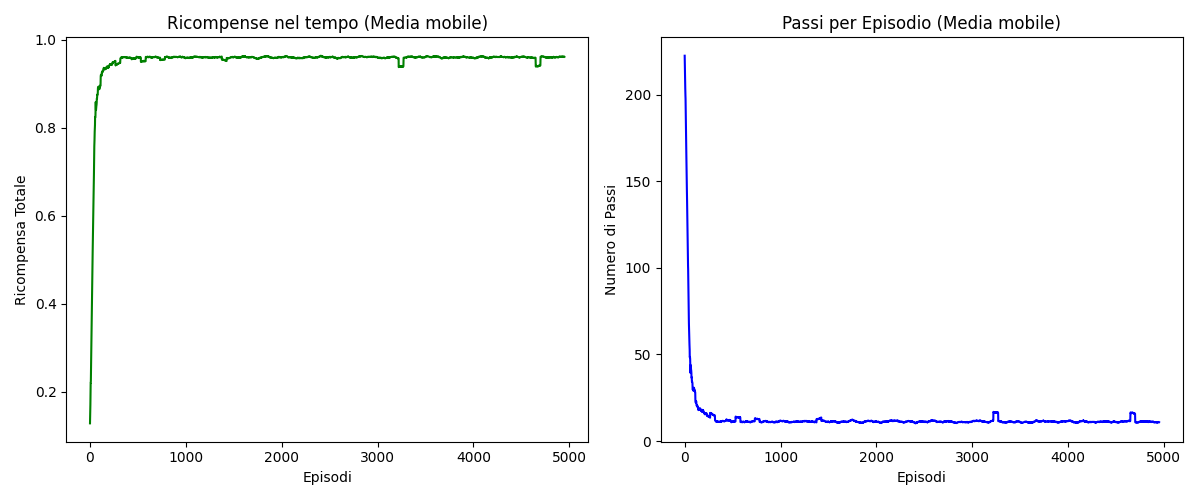
\includegraphics[width=\linewidth]{figure/Q-Learning/qtable1.png}
        \caption{Run 1}
    \end{subfigure}
    \hfill
    \begin{subfigure}{0.48\textwidth}
        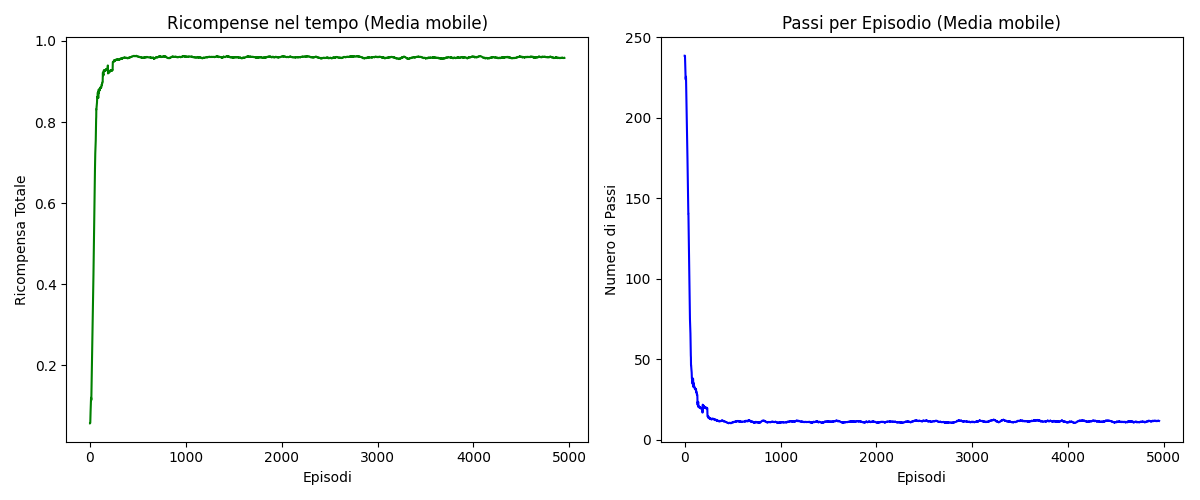
\includegraphics[width=\linewidth]{figure/Q-Learning/qtable2.png}
        \caption{Run 2}
    \end{subfigure}

    \vspace{1em}

    \begin{subfigure}{0.48\textwidth}
        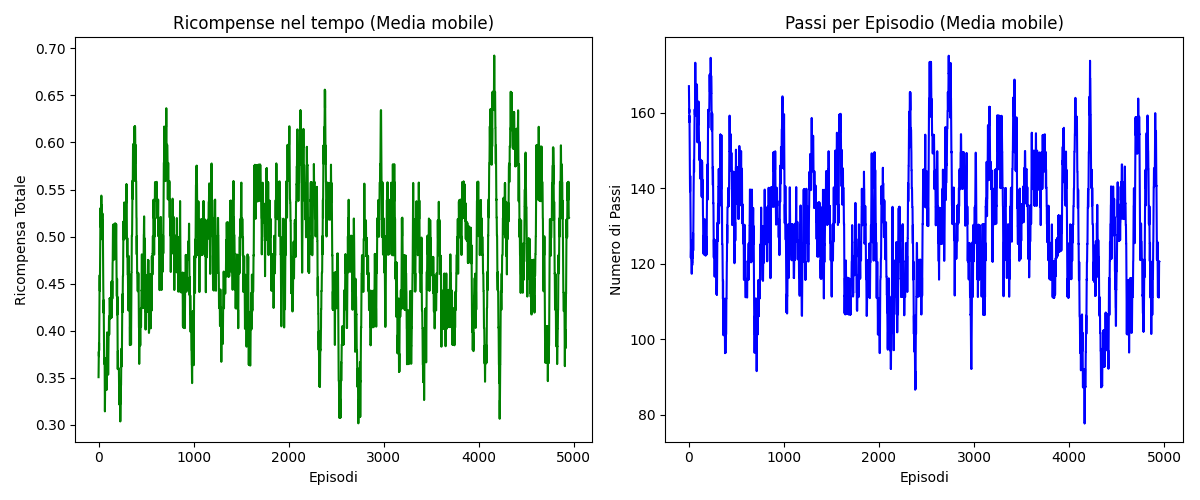
\includegraphics[width=\linewidth]{figure/Q-Learning/qtable3.png}
        \caption{Run 3}
    \end{subfigure}
    \hfill
    \begin{subfigure}{0.48\textwidth}
        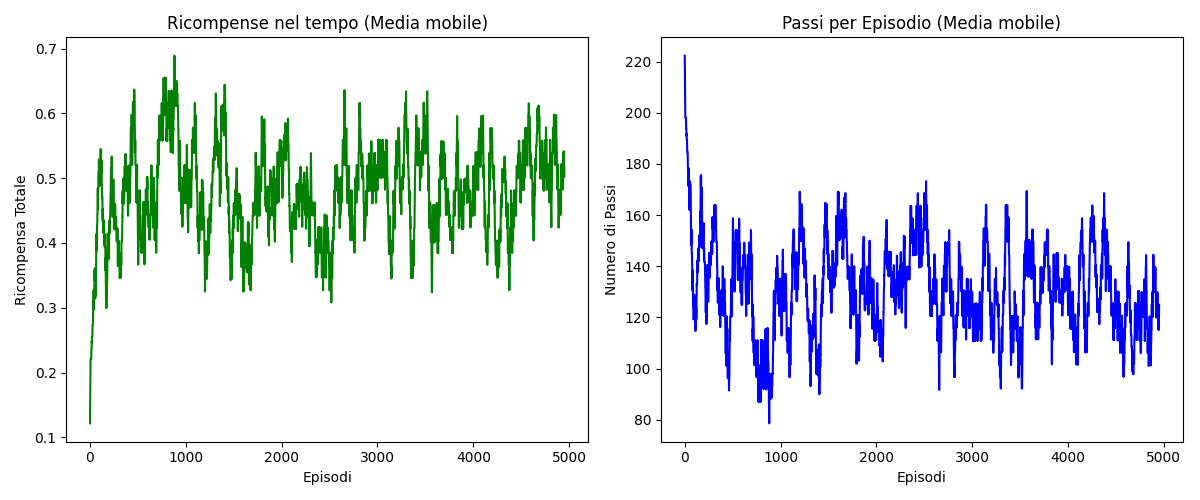
\includegraphics[width=\linewidth]{figure/Q-Learning/qtable4.png}
        \caption{Run 4}
    \end{subfigure}

    \vspace{1em}

    \begin{subfigure}{0.48\textwidth}
        \centering
        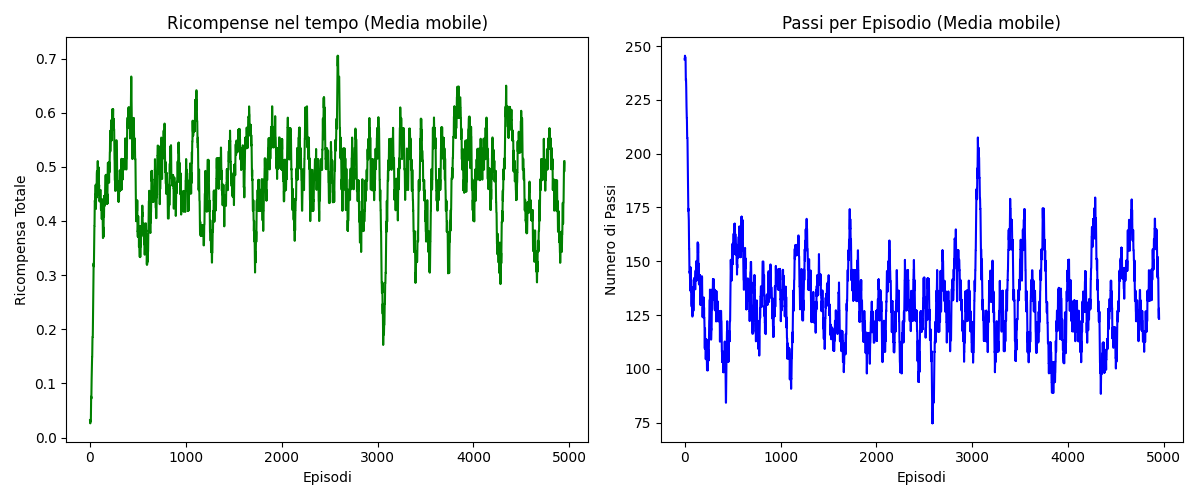
\includegraphics[width=\linewidth]{figure/Q-Learning/qtable5.png}
        \caption{Run 5}
    \end{subfigure}
    
    \caption{Risultati ottenuti con la Configurazione 1 ($\epsilon=0.9$, \texttt{max\_step}=250).}
    \label{fig:config1}
\end{figure}

% --- CONFIGURAZIONE 2 (Run 6-10) ---
\begin{figure}[htbp]
    \centering
    \begin{subfigure}{0.48\textwidth}
        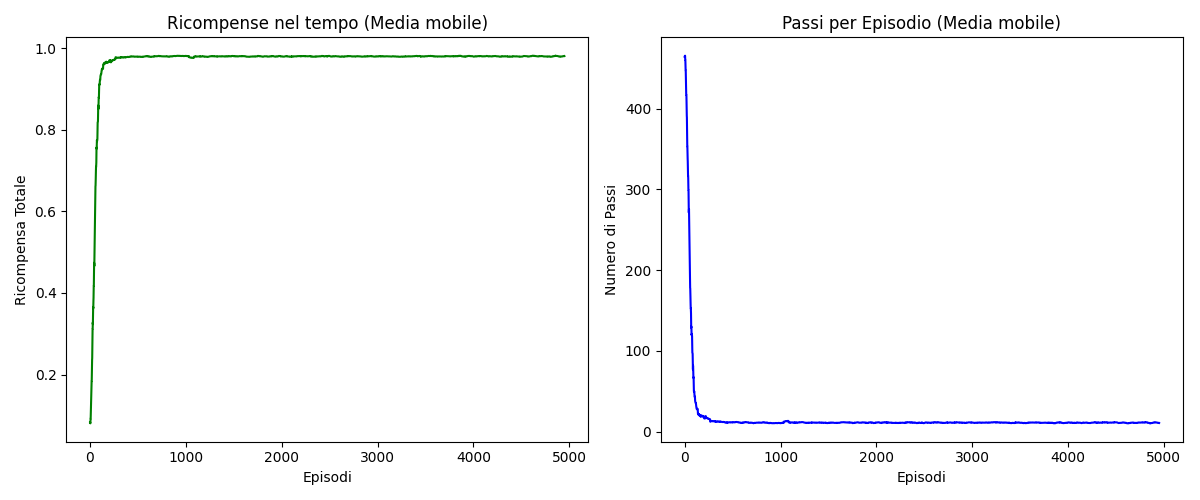
\includegraphics[width=\linewidth]{figure/Q-Learning/qtable6.png}
        \caption{Run 6}
    \end{subfigure}
    \hfill
    \begin{subfigure}{0.48\textwidth}
        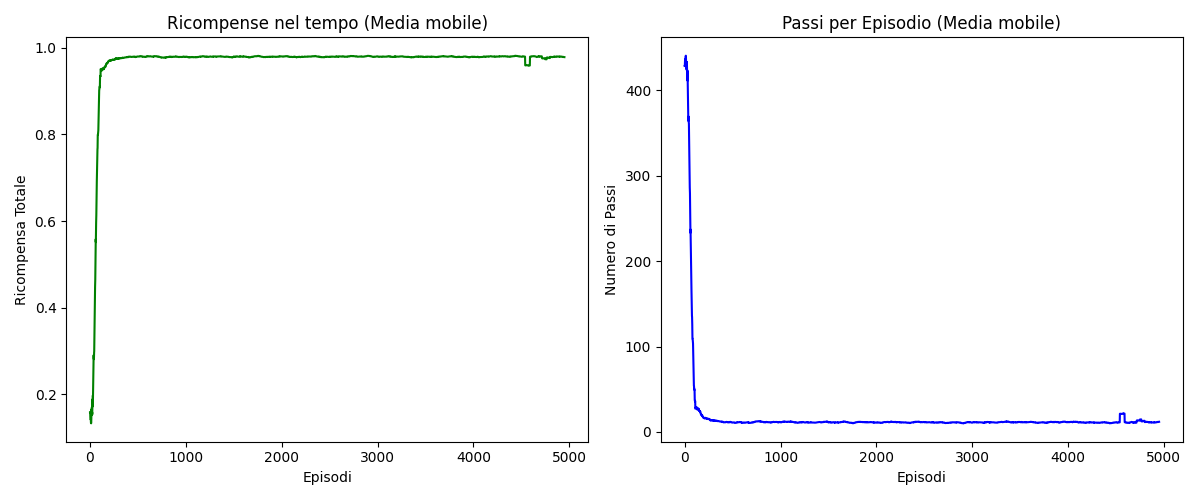
\includegraphics[width=\linewidth]{figure/Q-Learning/qtable7.png}
        \caption{Run 7}
    \end{subfigure}

    \vspace{1em}

    \begin{subfigure}{0.48\textwidth}
        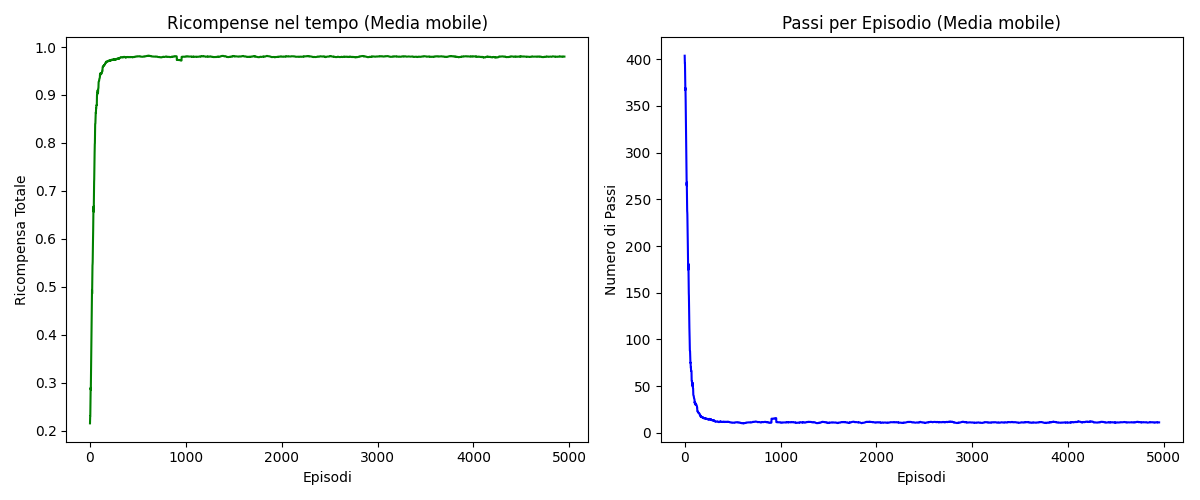
\includegraphics[width=\linewidth]{figure/Q-Learning/qtable8.png}
        \caption{Run 8}
    \end{subfigure}
    \hfill
    \begin{subfigure}{0.48\textwidth}
        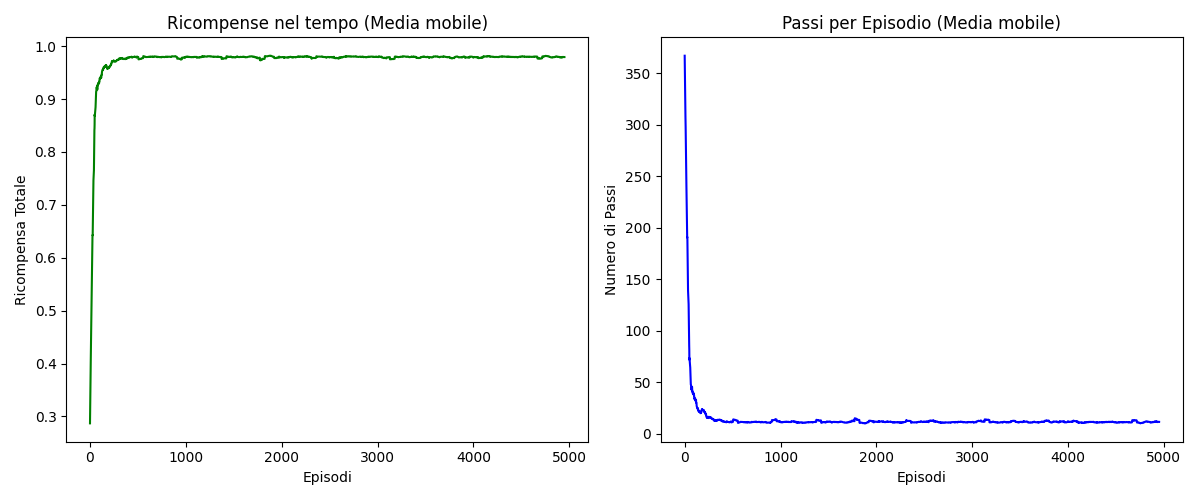
\includegraphics[width=\linewidth]{figure/Q-Learning/qtable9.png}
        \caption{Run 9}
    \end{subfigure}

    \vspace{1em}

    \begin{subfigure}{0.48\textwidth}
        \centering
        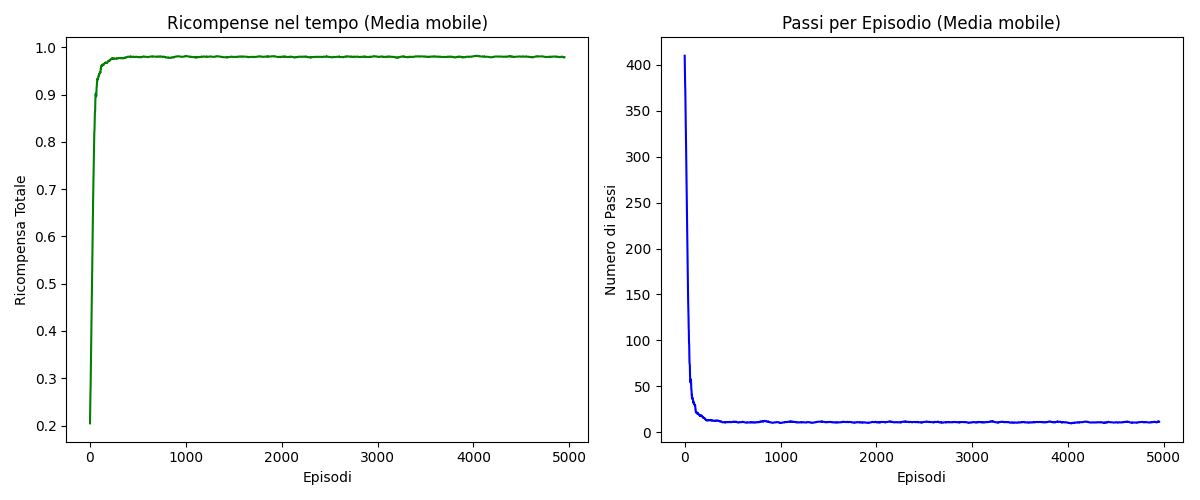
\includegraphics[width=\linewidth]{figure/Q-Learning/qtable10.png}
        \caption{Run 10}
    \end{subfigure}

    \caption{Risultati ottenuti con la Configurazione 2 ($\epsilon=1.0$, \texttt{max\_step}=500).}
    \label{fig:config2}
\end{figure}

\clearpage

\subsection{Analisi e Confronto delle Configurazioni}

Osservando i dati raccolti, emerge chiaramente che la \textbf{Configurazione 2} riesce a ottenere risultati ottimali e, soprattutto, ampiamente riproducibili nel tempo, a differenza della Configurazione 1 che mostra una maggiore instabilità o una convergenza verso policy sub-ottimali. 

Questo netto miglioramento delle performance è attribuibile a due fattori chiave:
\begin{enumerate}
    \item \textbf{Maggiore orizzonte temporale:} L'incremento del parametro \texttt{max\_step} da 250 a 500 fornisce all'agente il tempo materiale per completare con successo l'intera sequenza di azioni richieste dall'ambiente DoorKey (trovare la chiave, aprire la porta, raggiungere l'obiettivo) durante i primi episodi, quando i movimenti sono puramente stocastici.
    \item \textbf{Esplorazione massimizzata:} L'utilizzo di un tasso di esplorazione iniziale più elevato ($\epsilon = 1.0$) assicura che l'agente esplori a fondo l'ambiente prima di iniziare ad affidarsi alla policy appresa (\textit{exploitation}). In un ambiente a ricompensa sparsa come questo, esplorare maggiormente all'inizio previene la convergenza prematura e permette all'algoritmo di propagare correttamente i valori Q a ritroso dal goal fino agli stati iniziali.
\end{enumerate}


\end{document}